% IEEE standard conference template; to be used with:
%   spconf.sty  - LaTeX style file, and
%   IEEEbib.bst - IEEE bibliography style file.
% --------------------------------------------------------------------------

\documentclass[letterpaper]{article}
\usepackage{spconf,amsmath,amssymb,graphicx}

% Example definitions.
% --------------------
% nice symbols for real and complex numbers
\newcommand{\R}[0]{\mathbb{R}}
\newcommand{\C}[0]{\mathbb{C}}

% bold paragraph titles
\newcommand{\mypar}[1]{{\bf #1.}}

\newcommand{\fixme}[1]{{\bf FIXME}: {\it #1}}
\newcommand{\comment}[1]{}

\usepackage{amsmath}
\newcommand{\BigO}[1]{\ensuremath{\operatorname{O}\bigl(#1\bigr)}}

% Colors 
\usepackage{graphicx}
\usepackage[svgnames]{xcolor}
% URL
\usepackage[colorlinks=true,pdfborder={0 0 0},citecolor=DarkGreen,linkcolor=DarkBlue,urlcolor=DarkBlue]{hyperref}

% Code
\usepackage{listings}
\lstset{
    floatplacement={tbp},
    basicstyle=\ttfamily\mdseries\small,
    identifierstyle=,
    stringstyle=\color{gray},
    numbers=left,
    numbersep=5pt,
    inputencoding=utf8x,
    xleftmargin=8pt,
    xrightmargin=8pt,
    keywordstyle=[1]\bfseries,
    keywordstyle=[2]\bfseries,
    keywordstyle=[3]\bfseries,
    keywordstyle=[4]\bfseries,
    numberstyle=\tiny,
    stepnumber=1,
    breaklines=true,
    frame=lines,
    showstringspaces=false,
    tabsize=2,
    commentstyle=\color{gray},
    captionpos=b,
    float=float,
    language={Java}
}
\newcommand{\code}[1]{\lstinline{#1}}

% Title.
% ------
\title{Optimizing Domain Transform for Edge-Aware Image Processing}
%
% Single address.
% ---------------
\name{Adrian Blumer, Pascal Sp\"orri, Julia Pe\v{c}erska\comment{\thanks{The author thanks Jelena Kovacevic. This paper
is a modified version of the template she used in her class.}}} 
\address{Department of Computer Science\\ ETH Z\"urich\\Z\"urich, Switzerland}

\begin{document}
%\ninept
%
\maketitle
%
\begin{abstract}
\fixme{Review and shorten}

Edge-aware filtering can be used as a basic building block for many image processing tasks, for example colourisation of black and white images. However most of the algorithms existing for this task are unusable in real time as they require an extensive amount of complex computation.

This report discusses one of the fastest algorithms for such edge-aware filtering, which can be executed in linear time w.r.t. the number of pixels in the image. It uses a mapping (domain transform) from 5D image space (2 spatial dimensions and 3 colours) to 1D real space and an iterative approach to approximate the filtered image with sufficient precision.

In this report we describe the optimisation approaches which we used in order to further improve performance of this algorithm. We also provide a discussion of reasoning for several optimisation approaches which did not yield a significant increase in performance.

The baseline version of the implementation - the starting point for our optimisation - is a direct port of the matlab code provided by the authors of the algorithm. It precomputes values necessary for the filter, then alternates filter passes horizontally and vertically across the image while transposing the data representation between passes.

Overall after inlining and combining as many computation as possible, changing the image saving approach to writing in a fashion that can directly be read on the next iteration, and some vectorisation we managed to increase the performance of the code approximately $2$ times w.r.t. the baseline implementation, which is a good factor as the algorithm is rather efficient in the first place. Optimisation potential still exists as we are far from both memory and computation bounds, however neither of our further optimisation attempts got us closer to these bounds.

\comment{
Describe in concise words what you do, why you do it (not necessarily
in this order), and the main result.  The abstract has to be
self-contained and readable for a person in the general area. You
should write the abstract last.
}
\end{abstract}


\section{Introduction}\label{sec:intro}
\fixme{Review}

Filtering operations are often a crucial step of image processing and a particular sub-group of these are edge-aware smoothing filters. 
They are used as a basic building block for multiple other applications.
For example, such filters can be used to extract or remove features from an
image, to colorize the image in a intuitive fashion by colouring specific
items on an image, or to perform other tasks such as noise removal and
image compression ~\cite{GastalOliveira2011DomainTransform}.

As in most cases with image (and in particular with video) processing, it is highly required that the filters have a low computational cost and therefore can produce fast results. This is desireable to allow for real-time transformation of video streams as well as immediate feedback during image editing and in general when working on large datasets. 
It is also true that image recording technologies advance and therefore can create images of greater resolution, which means an increase in
the amount of computation needed for filtering.

\setlength\fboxsep{0pt}
\setlength\fboxrule{0.5pt}
 
\begin{figure}\vspace{-1mm}
  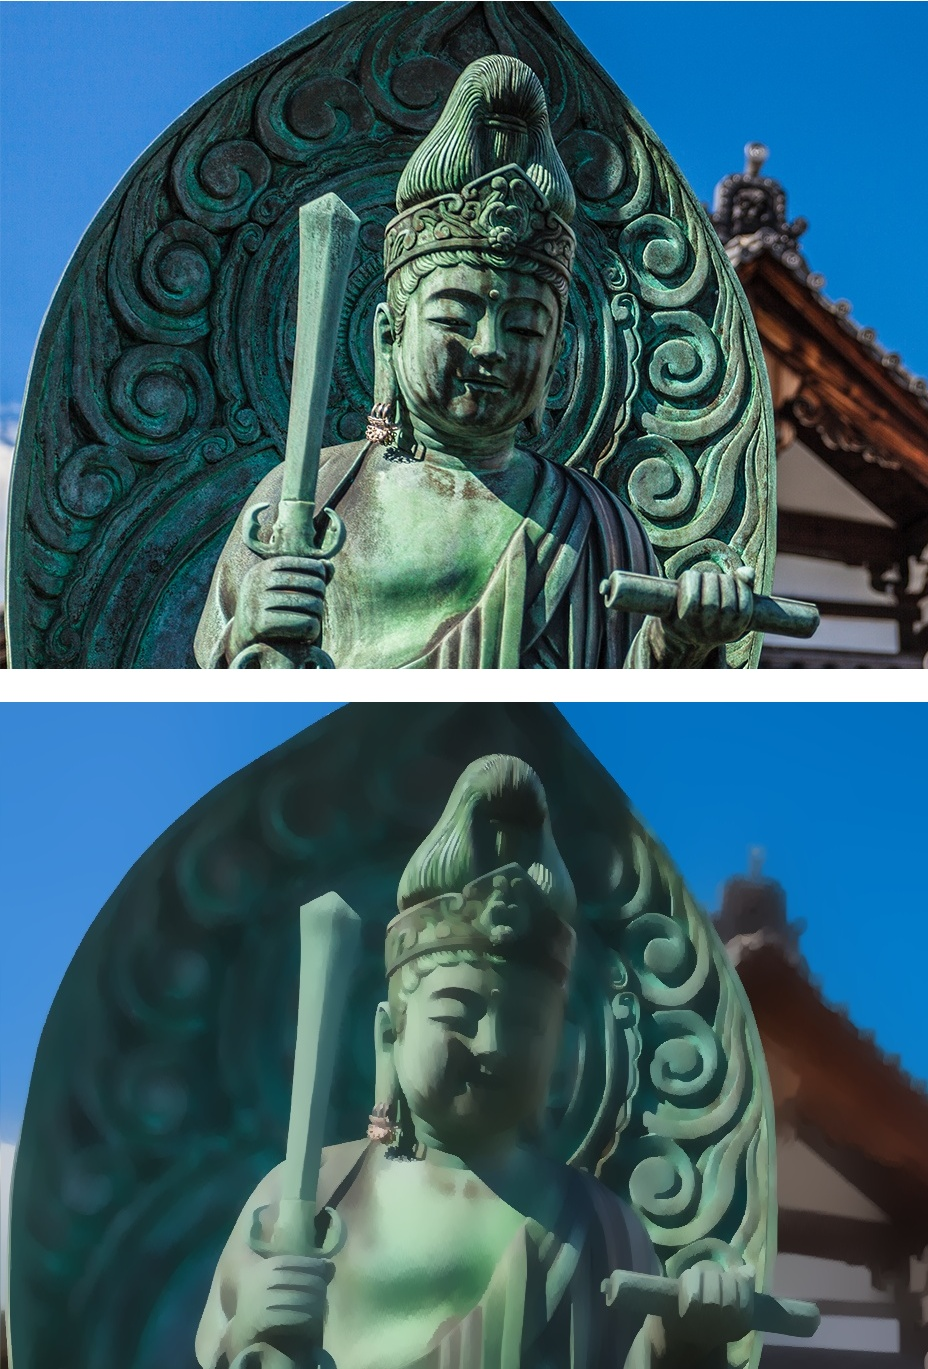
\includegraphics[trim=-30mm 0mm 0mm 0mm, clip, width=0.37\textwidth]{figures/input_output}
  \caption{Example input and output of our Normalized convolution implementation.\label{performance}}
\end{figure}


There exist multiple algorithms that perform this type of filtering, most of which fall into the categories of \textit{Bilateral filtering} and \textit{Anisotropic diffusion}. However most of these suffer either from quality, performance or scalability drawbacks. Moreover, some of them only naturally support grayscale images.

Recently, a new method that promises to solve these problems was prososed by Eduardo S. L. Gastal and Manuel M. Oliveira in their paper \textit{Domain Transform for Edge-Aware Image and Video Processing} ~\cite{GastalOliveira2011DomainTransform}.

This publication gives an in depth explanation of the theoretical foundations of the technique as well as presenting three different implementation approaches. These three approaches are called \textit{Normalized convolution} (NC), \textit{Interpolated convolution} (IC) and \textit{Recursive filtering} (RF).

So far the only publicly available implementation of these methods is done in MATLAB, published on the original papers homepage. While useful for verification and demonstration purposes, its runtime performance is far from optimal. The work presented here aims at providing an optimized implementation of the \textit{Normalized convolution} variant of the algorithm on the CPU while documenting the optimization process. We have implemented the algorith in C/C++ and proceeded to use the techniques described in the \textit{How to Write Fast Numerical Code} course ~\cite{HowToFastNumCode:2013:Webpage} to improve its performance.

\comment{Do not start the introduction with the abstract or a slightly modified
version. It follows a possible structure of the introduction. 
Note that the structure can be modified, but the
content should be the same. Introduction and abstract should fill at most the first page, better less.

\mypar{Motivation} The first task is to motivate what you do.  You can
start general and zoom in one the specific problem you consider.  In
the process you should have explained to the reader: what you are doing,
why you are doing, why it is important (order is usually reversed).

For example, if my result is the fastest DFT implementation ever, one
could roughly go as follows. First explain why the DFT is important
(used everywhere with a few examples) and why performance matters (large datasets,
realtime). Then explain that fast implementations are very hard and
expensive to get (memory hierarchy, vector, parallel). 

Now you state what you do in this paper. In our example: 
presenting a DFT implementation that is
faster for some sizes than all the other ones.

\mypar{Related work} Next, you have to give a brief overview of
related work. For a paper like this, anywhere between 2 and 8
references. Briefly explain what they do. In the end contrast to what
you do to make now precisely clear what your contribution is.
}
\section{Background: Whatever the Background is}\label{sec:background}
\fixme{Write.}

The original publication on the Domain Transform Filtering Technique ~\cite{GastalOliveira2011DomainTransform} gives  an in depth explanation of the theoretical foundations of the technique as well as presenting three different implementation approaches. These three approaches are called "Normalized convolution" (NC), "Interpolated convolution" (IC) and "Recursive filtering" (RF). 

In this section we will present the necessary background information to follow our implementation of the first of these three algorithms, namely "Normalized convolution". For a more detailed explanation of the method and it's background, please refer to the original publication.

The straight forward approach to image bluring is to compute a new value for each image pixel using the weighted average of its neighbourhood. To decide whether a pixel lies in this neighbourhood, we need some kind of distance measure. In the case of simple edge unaware bluring (such as applying a Gaussian filter), this distance measure is the spatial distance between image pixels. However to achieve edge-aware image filtering the radiometric distance between pixels (their difference in color) has to be taken into account as well.
In general this increases the dimensionality of the problem by adding a dimension for each color channel.

For a RGB color image this would lead to a 5-dimensional space (3 radiometric + 2 spatial dimensions). The domain transform method reduces this dimensionality as follows:
First, it threads the two spatial dimensions separately. What this means is that the images is separately filtered along its rows and columns. Secondly, it merges the three radiometric dimensions and the remaining one spatial dimension into the one-dimensional space of the domain transform, that still retains the necessary distance properties from the original space.


\mypar{Cost Analysis}
In asymptotic terms, the algorithm has a complexity of \BigO{n}, which makes it already very competitive with other approaches to edge-aware image filtering. For optimization purposes we are however interested in a more thorough cost analysis of the method. Therefore we have counted the number of different floating point operations executed by the algorithm:



\comment{
Give a short, self-contained summary of necessary
background information. For example, assume you present an
implementation of FFT algorithms. You could organize into DFT
definition, FFTs considered, and cost analysis. The goal of the
background section is to make the paper self-contained for an audience
as large as possible. As in every section
you start with a very brief overview of the section. Here it could be as follows: In this section 
we formally define the discrete Fourier transform, introduce the algorithms we use
and perform a cost analysis.

\mypar{Discrete Fourier Transform}
Precisely define the transform so I understand it even if I have never
seen it before.

\mypar{Fast Fourier Transforms}
Explain the algorithm you use.

\mypar{Cost Analysis}
First define you cost measure (what you count) and then compute the
cost. Ideally precisely, at least asymptotically. In the latter case you will need to instrument your code to count
the operations so you can create a performance plot.

Also state what is
known about the complexity (asymptotic usually) 
about your problem (including citations).

Don't talk about "the complexity of the algorithm.'' It's incorrect,
remember (Lecture 2)?
}
%\section{Your Proposed Method}\label{sec:method}
\section{Optimizing Domain Transform}
We started with the matlab code provided on the homepage\footnote{\url{http://www.inf.ufrgs.br/~eslgastal/DomainTransform/}} of the authors~\cite{GastalOliveira2011DomainTransform} and ported the code to C++. 
\subsection{Optimization Steps}
\subsubsection{Basic version}
In order to achieve the biggest optimisation potential the matrices have been wrapped in a simple struct (listing \ref{code:matrix_struct}).
\begin{lstlisting}[caption=Matrix struct,label=code:matrix_struct]
struct Mat2
{
    uint width, height;
    float3* data; // size: width*height
};
\end{lstlisting}
In order to preserve accuracy all images are stored in a \lstinline{float3} struct. Which uses $3\times 4 = 12$ bytes per pixel. Hence a $1$M pixel image is stored in $3\times 4\times 10^6$\ B $=12$\ MB.
The algorithm starts by precomputing $dIdx$ and $dIdy$ the differential of the image in both $x$ and $y$ direction. Then the prefix sum of both $dIdx$ and $dIdY^T$ is compute. 
During the filtering step we (listing \ref{code:filterstep}) compute \lstinline{computeBound} and \lstinline{boxFilter} twice. For each iteration step we transpose the images.
\begin{lstlisting}[caption=Filterstep,label=code:filterstep]
for (i=0; i<iterations; i++) {
    bounds = computeBound(img, dIdX, r);
    img = boxFilter(img, bounds);
    img = transpose(img);
    bounds = computeBound(img, dIdY, r);
    img = boxFilter(img, dIdY, bounds);
    img = transpose(img);
}
\end{lstlisting}
The \lstinline{computeBound} step computes the one dimensional bound for each pixel for the box filter step. The bound is dependant on a user defined radius $r$. 
During the box filter step the prefix sum of the image in the $x$ direction is precomputed with a separate function. During the box filter step the box filter makes use of the previously precomputed prefix sum and bounds to compute the filtered value for each pixel (listing \ref{code:boxfilter}).
\begin{lstlisting}[caption=Boxfilter step, label=code:boxfilter]
void boxfilter(img, bounds) {
    psum = prefixsum(img);
    for (i = 0; i < H; i++) {
        for (j = 0; j < W; j++) {
            l = lowerBound(i,j);
            r = upperBound(i,j);
            delta = r - l;
            img(i,j) = psum(l)-psum(r);
            img(i,j) = img(i,j)/delta;
        }
    }
}
\end{lstlisting}
\subsubsection{Blocked Transpose}
With benchmarking the initial version we recognised that the transpose function was responsible for most of our computation time. Hence we blocked the transpose (listing \ref{code:blocked_transpose}).
\begin{lstlisting}[caption=Transpose block, label=code:blocked_transpose]
for (yo=0; yo<Hmod; yo+=BLOCK)
  for (xo=0; xo<Wmod; xo+=BLOCK)
    for (uint y=yo; y<yo+BLOCK; y++)
      for (uint x=xo; x<xo+BLOCK; x++)
        uint idx = y*W + x;
        uint idxT = x*H + y;
        out.data[idxT] = in.data[idx];
    xo = Wmod;
    for (uint y=yo; y<yo+BLOCK; y++)
      for (uint x=xo; x<W; x++)
        uint idx = y*W + x;
        uint idxT = x*H + y;
        out.data[idxT] = in.data[idx];
// Handle bottom row and bottom rightmost block
\end{lstlisting}
\subsubsection{Inlining Bound Computation}
In order for compiler to optimise the the code we inlined the bound computation.
\begin{lstlisting}[caption=Inlining of the bound computation, label=code:inlining]
void boxfilter(img, dx, boxR) {
    psum = prefixsum(img);
    for (i=0; i<H; i++)
    {
        posL = 0;
        posR = 0;
        for (j=0; j<W; j++)
        {
            // Bound computation
            dtL = dx(i,j) - boxR;
            dtR = dx(i,j) + boxR;
            while (dx(i,posL) < dtL 
                    && posL < W-1)
                posL++;
            while (posR < W && 
                   dx(i,posR < dtR )
                posR++;
            // Boxfilter step
        }
    }
\end{lstlisting}
\subsubsection{Recombination}
The inlining allowed us to inline the prefix sum into the boxfilter bound computation step (listing \ref{code:recombination}).
\begin{lstlisting}[caption=Recombination, label=code:recombination]
    while (dx(i,posL) < dtL 
            && posL < W-1)
        sum -= imgRow[posL];
        posL++;

    while (posR < W && 
           dx(i,posR < dtR )
        sum  += imgRow[posR];
        posR++;
    // Boxfilter step
    invD = 1.0f /(posR-posL);
    img(i,j) = sum * invD;
\end{lstlisting}
\subsubsection{Write transpose}
By directly storing the data transposed with were able to increase performance and reduce the number of transpose functions needed to be computed. We note that 

\subsection{Failed optimization attempts}

\fixme{Rewrite}
\subsubsection{Precomputation} Division precomputation did not make any difference.

\subsubsection{Changing floats to \dots}

\fixme{Write}

\subsubsection{Blocking}

We tried to block the computation for spatial locality for the output matrix which didn't give any improvement (actually made it worse).

\subsubsection{Instruction interleaving}

We tried to combine the while loops that compute the borders for the filter, so that independent computation would fill the pipeline. This did not give any performance improvement, perhaps because of the fact that the combined loop still had a conditional statement for both filter borders which we cannot eradicate.

\subsubsection{Reshuffling of data}

Most of the versions we implemented work on the interleaved colour arrays, storing colours as $rgbrgb\dots$. We attempted to reshuffle the data to three separate arrays, each containing one colour, which didn't bring any performance improvement. 

We transpose 3 different arrays which is slow. Or we might write transposed, but then we'd access 3 arrays at a stride which would mess the cache up anyway.

%\\
%\fixme{Write.}
%\comment{
%Now comes the ``beef'' of the paper, where you explain what you
%did. Again, organize it in paragraphs with titles. As in every section
%you start with a very brief overview of the section.
%
%For this class, explain all the optimizations you performed. This mean, you first very briefly
%explain the baseline implementation, then go through locality and other optimizations, and finally SSE (every project will be slightly different of course). 
%Show or mention relevant analysis or assumptions. A few examples: 
%1) Profiling may lead you to optimize one part first; 
%2) bandwidth plus data transfer analysis may show that it is memory bound; 
%3) it may be too hard to implement the algorithm in full generality: make assumptions and state them 
%(e.g., we assume $n$ is divisible by 4; or, we consider only one type of input image); 
%4) explain how certain data accesses have poor locality. Generally, any type of analysis adds value to your work.
%
%As important as the final results is to show that you took a structured, organized approach to the optimization and that you explain why you did what you did.
%
%Mention and cite any external resources including library or other code.
%
%Good visuals or even brief code snippets to illustrate what you did are good. Pasting large amounts of code to fill the space is not good.
%}
\section{Experimental Results}\label{sec:exp}
\subsection{Experimental Setup}\label{sec:exp_setup8}
In order to test and benchmark the code we stored each major benchmark revision in a separate folder. Then we run a script that compiled the code and benchmarked it against $5$ different image sizes (figure \ref{tab:images}). The image sizes were chosen in such a way that they represent real world applications used in an image processing or video processing software. The images \texttt{bhudda\_200.png} and \texttt{bhudda\_300.png} have been chosen since both fit into the L3 cache. 
\begin{figure}
\centering
{\small
\begin{tabular}{rll}
\textbf{Image} & \textbf{Size}\\
\texttt{bhudda\_200.png} & $0.02$ & Megapixel\\
\texttt{bhudda\_320.png} & $0.07$ & Megapixel\\
\texttt{bhudda\_640.png} & $0.26$ & Megapixel\\
\texttt{bhudda\_720p.png} & $0.92$ & Megapixel\\
\texttt{bhudda\_1080p.png} & $2.07$ & Megapixel\\
\end{tabular}
}
\caption{Images used for benchmarking}
\label{tab:images}
\end{figure}

\subsubsection{Platform}
Benchmarking was done on a Ubuntu Linux 12.10 running on a Intel Core i7-3610QM "Ivy Bridge" CPU. In order to generate repeat reproducible results the CPU frequency was set to $2.3$ GHz with Turbo Boost disabled.
\subsubsection{Tools and counters used}
The code was both compiled and executed on GCC 4.6.4 and ICC 13.1.2.183 64bit. We found that the compiler flags \lstinline{-O3 -march=corei7} produced optimal results in our case. In the results shown we only show results obtained with GCC since the ICC results show the same performance measurements. We noticed that code generated with the compiler flags \lstinline{-O3 -march=corei7-avx} was slower. Since the compiler used the \lstinline{vaddps} instruction with 3 input values. Whereas the \lstinline{-O3 -march=corei7} only add the \lstinline{addps} instruction which uses 2 input values and thus reduces the code size and helps with branch miss predictions since there's less code to load. 

To measure the performance we used a custom timing framework using RTDSC counters. For additional checks we used Intel VTune 2013\footnote{\url{http://software.intel.com/en-us/intel-vtune-amplifier-xe}}. In order to generate the roofline plots (figure \ref{roofline}) we used the perfplot tool\footnote{\url{https://github.com/GeorgOfenbeck/perfplot}} provided by Georg Ofenbeck. To measure the memory bandwith of the reference computer we used Bandwith\footnote{\url{http://zsmith.co/bandwidth.html}}.
\subsection{Results}
We were able to achieve a speedup of $1.98$ for the cache based image \texttt{bhudda\_320.png} with a performance of $0.38$ flops/cycle and a speedup $2.24$ for our HD style image \newline\texttt{bhudda\_1080p.png} with a total performance of $0.32$ flops/cycle (figure \ref{performance}). In our roofline plot \cite{Williams:2009:RIV:1498765.1498785} (figure \ref{roofline}) we observe that we read/write bound for our \texttt{bhudda\_1080p.png} image denoted as \textbf{1080} in the plot. As soon as we decrease the image size (\textbf{720} denotes the image \texttt{bhudda\_720p.png}, \textbf{640} denotes the image \texttt{bhudda\_640.png}, \textbf{320} denotes the image \texttt{bhudda\_320.png}, \textbf{200} denotes the image \texttt{bhudda\_200.png}) we observe that the operational intensity changes but not the performance of the code (figure \ref{roofline}). Hence there must be another limiting factor. 

\setlength\fboxsep{0pt}
\setlength\fboxrule{0.5pt}
 
\begin{figure}\vspace{-10mm}
  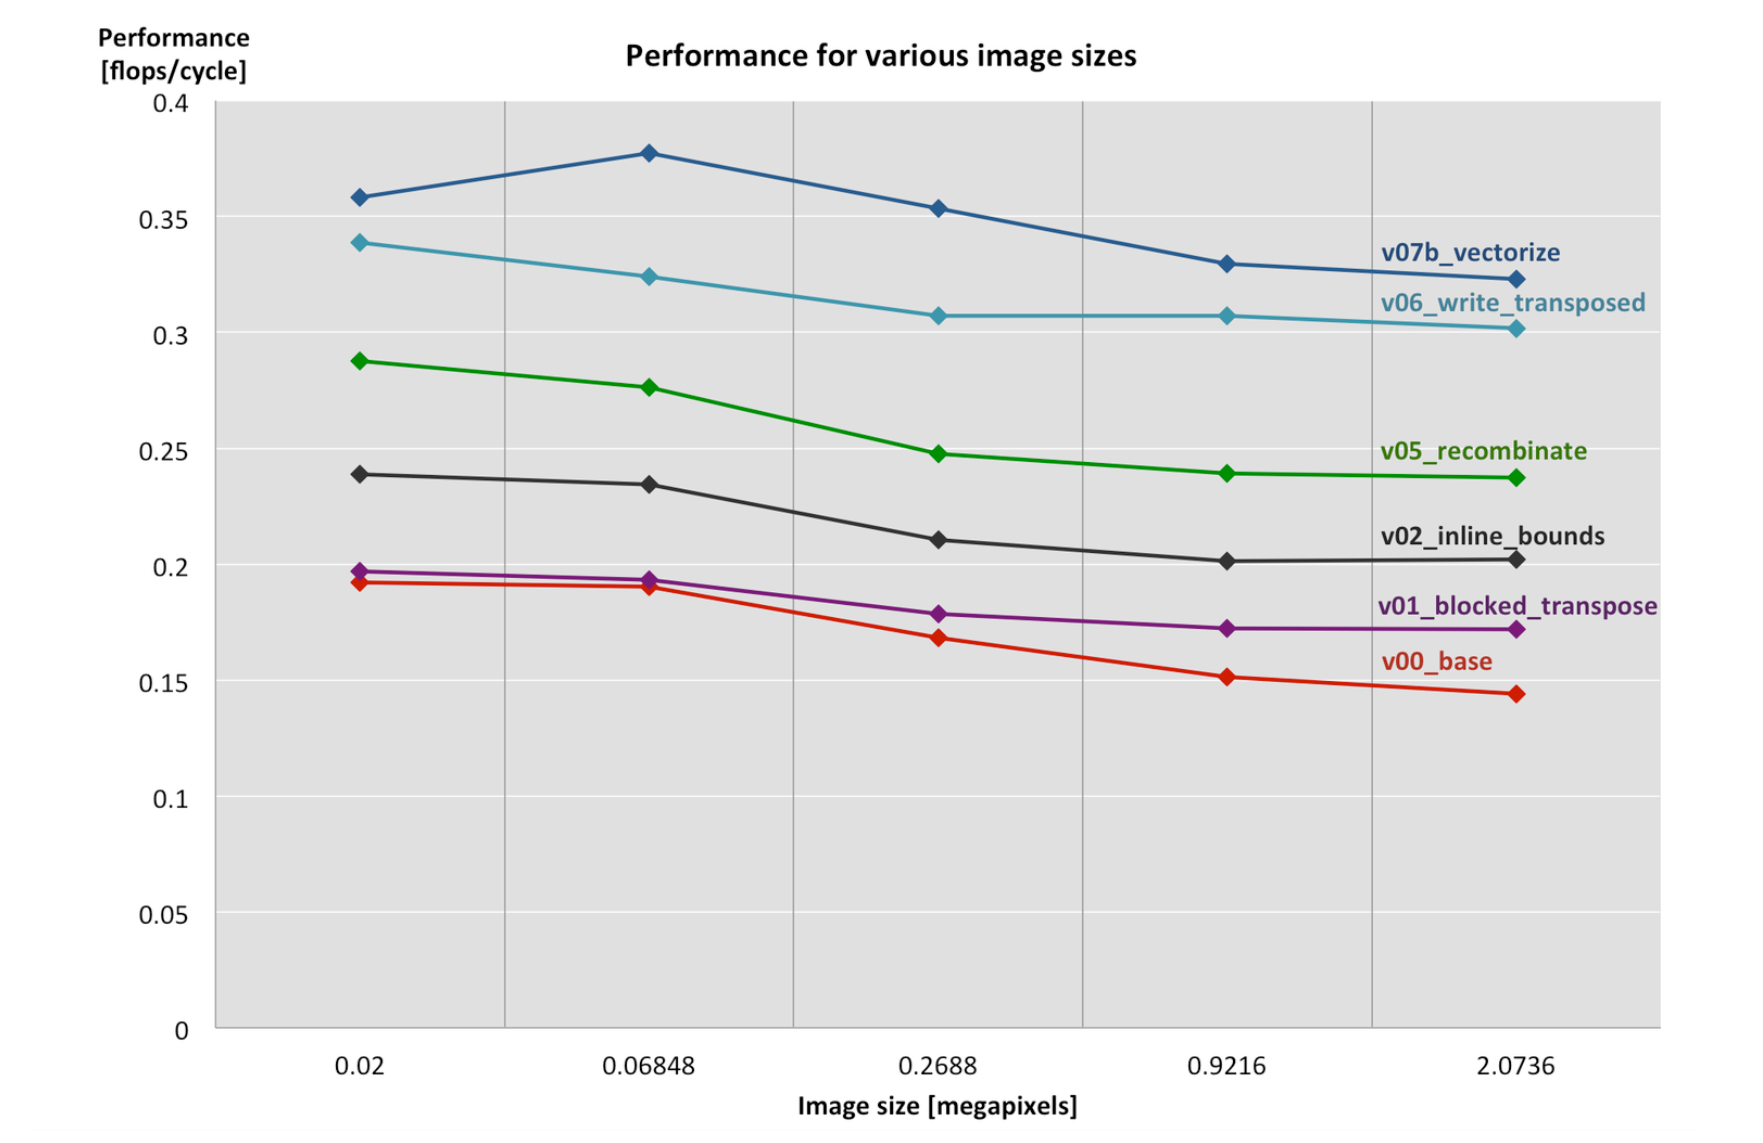
\includegraphics[trim=10mm 0mm 10mm 0mm, clip, width=0.49\textwidth]{figures/performance}
  \caption{Performance plot comparing our different optimisation levels. Compiler: GCC 4.6.4, flags: \lstinline{-O3 -march=corei7}.\label{performance}}
\end{figure}
 
\begin{figure}\vspace{-6mm}\hspace{-5mm}
%  \includegraphics[trim=10mm 0mm 10mm 0mm, clip, width=0.49\textwidth]{figures/roofline}
  \includegraphics[width=0.55\textwidth]{figures/roofline}
  \caption{Roofline plot showing the performance of our vectorised code. Compiler: GCC 4.6.4, flags: \lstinline{-O3 -march=corei7}.\label{roofline}}
\end{figure}


\comment{
Here you evaluate your work using experiments. You start again with a
very short summary of the section. The typical structure follows.

\mypar{Experimental setup} Specify the platform (processor, frequency, cache sizes)
as well as the compiler, version, and flags used. I strongly recommend that you play with optimisation flags and consider also icc for additional potential speedup.

Then explain what input you used and what range of sizes. The idea is to give enough information so the experiments are reproducible by somebody else on his or her code.

\mypar{Results}
Next divide the experiments into classes, one paragraph for each. In the simplest case you have one plot that has the size on the x-axis and the performance on the y-axis. The plot will contain several lines, one for each relevant code version. Discuss the plot and extract the overall performance gain from baseline to best code. Also state the percentage of peak performance for the best code. Note that the peak may change depending on the situation. For example, if you only do additions it would be 12 Gflop/s
on one core with 3 Ghz and SSE and single precision floating point.

Do not put two performance lines into the same plot if the operations count changed significantly (that's apples and oranges). In that case first perform the optimisations that reduce op count and report the runtime gain in a plot. Then continue to optimise the best version and show performance plots.

{\bf You should}
\begin{itemize}
\item Follow the guide to benchmarking presented in class, in particular
\item very readable, attractive plots (do 1 column, not 2 column plots
for this class), proper readable font size. An example is below (of course you can have a different style),
\item every plot answers a question, which you pose and extract the
answer from the plot in its discussion
\end{itemize}
Every plot should be discussed (what does it show, which statements do
you extract).
}
\section{Conclusions}
\fixme{Write.}

In this report we presented a summary of optimization strategies for an edge preserving blurring filter. Even though the baseline implementation was already fast, we got an approximate $2x$ peformance gain in our final code version.

During the course of optimization we got rid of the primitive bottleneck which was the matrix transpose, by writing the data in transposed fashion directly. This allowed us to focus on the iterative part of the algorithm.

The way data is processed gives natural spatial locality and also instruction level paralellism, as 3 colour channels are stored contiguously but computed independently. This is also the reason why manual vectorization didn't give any performance improvement, as the pipeline of computation was already filled as much as the data allows.

We have attempted to analyze the performance bound of our code using roofline plots. However our fastest version is neither memory or compute bound, as we can see from the plot. This probably means that we are bound by some other factor. \comment{which we have no idea what it is :b}

\comment{
Here you need to briefly summarize what you did and why this is
important. {\em Do not take the abstract} and put it in the past
tense. Remember, now the reader has (hopefully) read the paper, so it
is a very different situation from the abstract. Try to highlight
important results and say the things you really want to get across
(e.g., the results show that we are within 2x of the optimal performance ... 
Even though we only considered the DFT, our optimization
techniques should be also applicable ....) You can also formulate next
steps if you want. Be brief.
}

%\vspace{-5mm}
\bibliographystyle{IEEEbib}
\bibliography{bibl_conf}

\end{document}

